% 1988_guangdong_science_q26_fig1: square pyramid P-ABCD
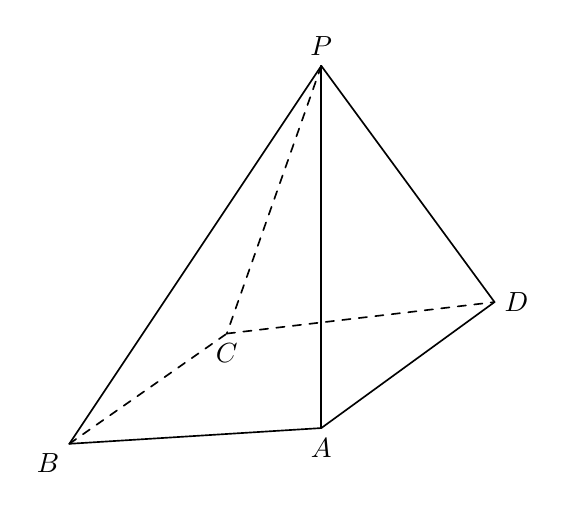
\begin{tikzpicture}[line width=0.6pt, line join=round, line cap=round]
\coordinate (P) at (0.6,3.2);
\coordinate (B) at (-2.6,-1.6);
\coordinate (A) at (0.6,-1.4);
\coordinate (D) at (2.8,0.2);
\coordinate (C) at (-0.6,-0.2);
% solid lateral + base front edges
\draw (P) -- (B);
\draw (P) -- (A);
\draw (P) -- (D);
\draw (B) -- (A);
\draw (A) -- (D);
% hidden dashed
\draw[dashed] (P) -- (C);
\draw[dashed] (B) -- (C);
\draw[dashed] (C) -- (D);
% labels
\node[above] at (P) {$P$};
\node[below left] at (B) {$B$};
\node[below] at (A) {$A$};
\node[right] at (D) {$D$};
\node[below] at (C) {$C$};
\end{tikzpicture}
